%++++++++++++++++++++++++++++++++++++++++
% Don't modify this section unless you know what you're doing!
\documentclass[letterpaper,11pt]{article}
\usepackage{natbib}
\bibliographystyle{unsrtnat}
\usepackage{tabularx} % extra features for tabular environment
\usepackage{amsmath}  % improve math presentation
\usepackage{graphicx} % takes care of graphic including machinery
\usepackage[margin=1in,letterpaper]{geometry} % decreases margins
%\usepackage{cite} % takes care of citations
\usepackage[final]{hyperref} % adds hyper links inside the generated pdf file
\hypersetup{
	colorlinks=true,       % false: boxed links; true: colored links
	linkcolor=blue,        % color of internal links
	citecolor=blue,        % color of links to bibliography
	filecolor=magenta,     % color of file links
	urlcolor=blue         
}
%+++++++++++++++++++++++++++++++++++++++
\begin{document}

\title{Course No. and Lab No. \\\textbf{Customer Personality Analysis}}
\author{G0: S. Chung, et. al.}
\date{January 1, 2050}
\maketitle

\begin{abstract}
(Sample only) Theoretical models for varying ... for the ... produced by ... were determined using ... Measurements were performed using ... and ... by means of ... Analyses were performed using techniques in ... and mathematical tools such as ... It has been found that ... $\vec{B}= (1.11 \pm 0.02)\times10^5\text{T}$ ...which agrees with the theoretical value of ... within errors. The precision/accuracy of [equipment/method] was not ... Fitting parameters of ... suggest that ...systematic errors, random errors... and that [these] should have been accounted for, etc. 
\end{abstract}

\section{Introduction}

(Sample only, note the functions in bold-facing, italics, etc.) \\In 1820, \textbf{Biot and Savart} conducted an experiment in ... [1]. 

The \textit{Biot-Savart Law} is useful in ... [2].

A \textcolor{blue}{Helmholtz coil} is a device for ... and was named after ... These coils were widely used in ... to produce \underline{uniform magnetic fields} ...

The objective in this present lab is to ...

\section{Theory}

State, derive, and describe the important equations that you will need to use to compare theory and experiment. Include diagrams as necessary to help with visualizing variables. Leave mathematical details of your derivations on the Appendix section. Below is an example to insert a numbered equation \ref{eq1} below

\begin{equation} \label{eq1} % the label is used to reference the equation
V=\frac{8\phi\Delta\pi a^{-5}}{\sqrt{3}\lambda\alpha\cdot\delta X \cdot\Sigma}+\nabla\vec{B}+\frac{\vec{E}}{\vec{v}}+\int \psi dL
\end{equation}

where $\psi$ is the distance to the Sun in units of km, $\lambda$ is something ... Always explain each variable once introduced. Do not introduce again at a later paragraph. 

Example on how to insert an equation on a separate line, unnumbered:
$$s_f=s_0+v_0t+\frac{1}{2}at^2$$
or you can state equations or variables within the paragraph like this $v_f^2=v_i^2+2a\Delta s$ or variable $\xi$.

\section{Methods}
Introduce all the steps and the equipment you used in the experiment. List or tabulate as necessary. Include model numbers, diagrams, schematics, all with labels. Make sure that the method is listed sufficiently such that someone else can easily replicate your experiment.

Include diagrams/photos of the experimental setup (see Figure \ref{fig1}) (Note that referencing a figure comes before actually showing the figure!), or screenshots highlighting important steps of the process. Make sure it is large enough to see the whole picture; crop the picture and remove non-important spots.

\begin{figure}[ht] 
        \centering 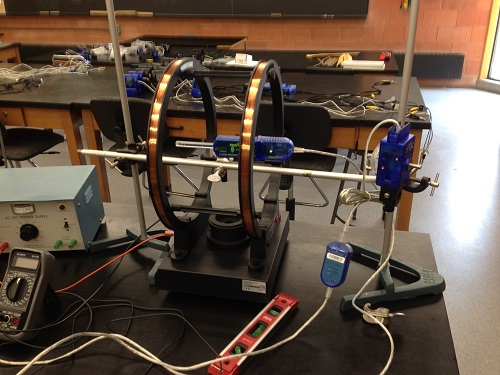
\includegraphics[width=0.9\columnwidth]{HCoil}
        \caption{\label{fig1}Every figure MUST have a caption. Note that the figure caption is below the figure! You should also label the instruments above, say, (a) Coils, (b) DMM, etc.
        }
\end{figure}

\section{Results and Analysis}

Describe all your results after presenting them. Include tabulated data set, larger tables can also be presented on the Appendix. Here's an example to insert a table -  Table~\ref{table1} is below:

\begin{table}[ht]
\begin{center}
\caption{Every table needs a caption. Note that the table caption is on top of the table! Note the consistency of precision of table values; do not forget the errors, labels, variables, and units.}
\label{table1} 
\begin{tabular}{ccc} %change to cc for 2 columns
\hline
\multicolumn{1}{c}{Distance, $d$ (km) } & \multicolumn{1}{c}{Voltage, $V\ (\pm 0.05$ V)} & \multicolumn{1}{c}{Current, $I$\ (mA $\pm 5$\%)}\\
\hline
1.2 $\pm$ 0.2 &  0.30 & 20 \\
1.6 $\pm$ 0.4 &  0.21 & 30 \\
2.5 $\pm$ 0.1 &  0.18 & 40 \\
5.9 $\pm$ 0.2 &  0.13 & 50 \\
\hline
\end{tabular}
\end{center}
\end{table}

\textbf{Use a full page to present important plotted findings, \textcolor{red}{don't be shy!}}(See Appendix for e.g.). Your plots should have axes labels with units, error bars, legend, captions, etc.

You can also discuss the sources of errors in this section; include ways on how you may want to improve the experimental methods performed. 



\section{Conclusion}
This section should be brief, concise, but complete. Directly answer your objectives, state your findings with errors, and conclude whether or not you were successful. Briefly explain if not successful.

\begin{thebibliography}{99}

\bibitem[\protect\citeauthoryear{Author}{2010}]{Author2010}
Author, A.N and Another, A. N., 2010, MNRAS, 431, 28.

\end{thebibliography}

\appendix

\section*{Appendix: Velocity measurements}

Below is an example large table; include mathematical derivations here as well.
\begin{table}[ht]
\begin{center}
\caption{Every table needs a caption.}
\label{table2} 
\begin{tabular}{cc} 
\hline
\multicolumn{1}{c}{distance (m)} & \multicolumn{1}{c}{V (km s$^-1$)} \\
\hline
0.0044151 &   0.0030871 \\
0.0021633 &   0.0021343 \\
0.0003600 &   0.0018642 \\
0.0023831 &   0.0013287 \\
0.0044151 &   0.0030871 \\
0.0021633 &   0.0021343 \\
0.0003600 &   0.0018642 \\
0.0023831 &   0.0013287 \\
0.0044151 &   0.0030871 \\
\hline
\end{tabular}
\end{center}
\end{table}

See the inserted full page plot below (Figure \ref{fig2}) for reference (sample data only, past student submission).

\begin{figure}[ht] 
        \centering 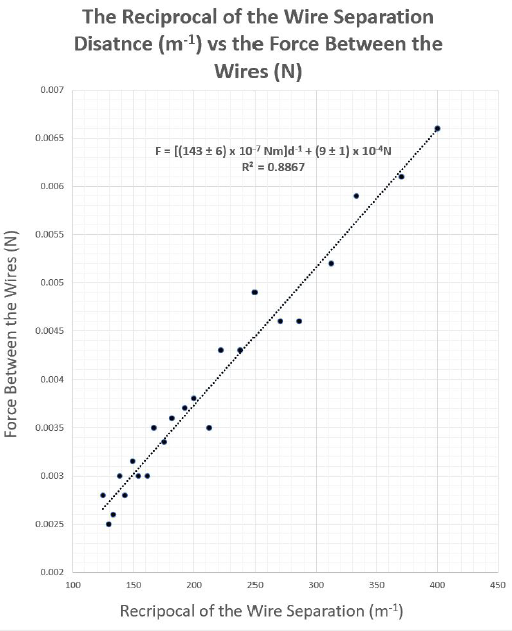
\includegraphics[width=.9\columnwidth]{Capture}
        \caption{\label{fig2}Every figure MUST have a caption. Note that the figure caption is below the figure! Do not foget to include error bars on your plots.
        }
\end{figure}


\end{document}
